\chapter{xHCI Stack Implementation}

The structure of the xHCI driver is quite straightforward, as it tries to fit
into the scheme of how hardware and the rest of HelenOS works. We decided to
use the existing library \lib{libusbhost} to reduce code duplication with
other HC drivers. IT came out that this library need a lot of changes to
support us in this goal, but that's for chapter \ref{usb-refactoring}.

The USB host controller driver using libusbhost, xHCI included, serves as
a connecting layer between the hardware and librabry, and exposes its bus
interface.

\begin{figure}[h]
	\centering
	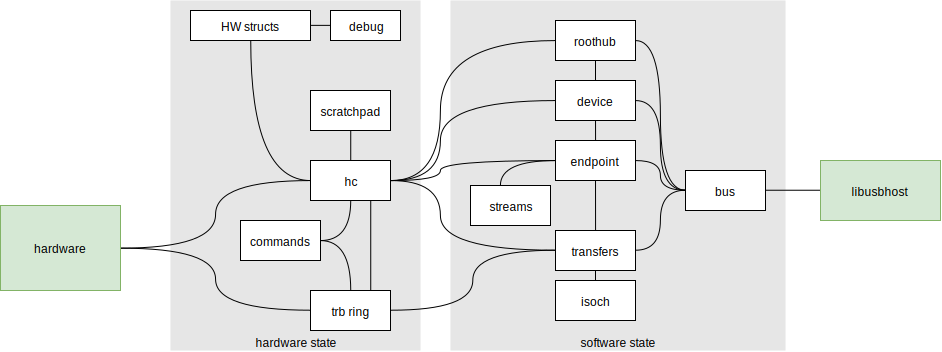
\includegraphics[width=0.8\textwidth]{xhci-architecture}
	\caption{The modules of xHCI driver}
\end{figure}
